% questions.tex —— 2013 年·北京卷·理科 · 题目内容片段（无答案）
% 由 tools/generate_projects.py 依来源总账自 2013/2013_数学真题_北京理_试题.md 生成，勿手改（改源 MD 后重跑）


\begin{gknotice}
\textbf{来源说明}：本题面依据固定源 PDF 的两页 A3 题面逐题转录，原卷印刷页码为 787—788。第 787 面为选择题 1—8、填空题 9—14、解答题 15—16，第 788 面为解答题 17—20。原卷无选做栏。

\textbf{解析归属}：固定源不附答案或解析；配套答案与解析均由本库按本题面独立复算。

\textbf{图形说明}：第 4 题程序框图、第 11 题圆的切线与割线、第 13 题正方形网格中的向量、第 14 题正方体、第 16 题空气质量指数趋势图、第 17 题三棱柱，均由项目内 TikZ 矢量源重绘。
\end{gknotice}

\gkpart{一、选择题}

\begin{question}
\gkti{1}已知集合 $A=\{-1,0,1\}$，$B=\{x\mid-1\leqslant x<1\}$，则 $A\cap B=$\mbox{（　　）}

（A）$\{0\}$；（B）$\{-1,0\}$；（C）$\{0,1\}$；（D）$\{-1,0,1\}$。

\end{question}
\begin{question}
\gkti{2}在复平面内，复数 $(2-\mathrm i)^2$ 对应的点位于\mbox{（　　）}

（A）第一象限；（B）第二象限；（C）第三象限；（D）第四象限。

\end{question}
\begin{question}
\gkti{3}“$\varphi=\pi$”是“曲线 $y=\sin(2x+\varphi)$ 过坐标原点”的\mbox{（　　）}

（A）充分而不必要条件；（B）必要而不充分条件；（C）充分必要条件；（D）既不充分也不必要条件。

\Needspace{0.4\textheight}
\end{question}
\begin{question}
\gkti{4}执行如图所示的程序框图，输出的 $S$ 值为\mbox{（　　）}
\nopagebreak[4]
\begin{center}% 2013 年北京卷理科第 4 题：程序框图。
% 来源 PDF：普通高考/2013/2013北京理.pdf，第 1 页（印面 787）左栏。
% 流程：开始 → i=0,S=1 → S=(S^2+1)/(2S+1) → i=i+1 → i≥2?
%       是：输出 S → 结束；否：回到 S 赋值框。
\begin{tikzpicture}[font=\footnotesize, >=Stealth, line width=0.45pt,
  node distance=4.5mm,
  term/.style={draw, rounded corners=6pt, minimum height=1.8em, inner xsep=9pt},
  io/.style={draw, trapezium, trapezium left angle=70, trapezium right angle=110,
             minimum height=1.8em, inner xsep=6pt},
  box/.style={draw, minimum height=1.9em, inner xsep=6pt},
  dec/.style={draw, diamond, aspect=2.2, inner sep=1pt}]
  \node[term] (start) {开始};
  \node[box, below=4mm of start] (init) {$i=0$，$S=1$};
  \node[box, below=4mm of init] (assign) {$S=\dfrac{S^2+1}{2S+1}$};
  \node[box, below=4mm of assign] (inc) {$i=i+1$};
  \node[dec, below=5mm of inc] (cond) {$i\geqslant 2$};
  \node[io, right=16mm of cond] (output) {输出 $S$};
  \node[term, below=5mm of output] (end) {结束};
  \draw[->] (start) -- (init);
  \draw[->] (init) -- (assign);
  \draw[->] (assign) -- (inc);
  \draw[->] (inc) -- (cond);
  \draw[->] (cond) -- node[above] {是} (output);
  \draw[->] (output) -- (end);
  % 循环支路：从判断框左侧引出，向上回到 S 赋值框左侧
  \draw[->] (cond.west) -- node[above] {否} ++(-2.1,0) |- (assign.west);
\end{tikzpicture}
\end{center}
\nopagebreak[4]
（A）$1$；（B）$\dfrac23$；（C）$\dfrac{13}{21}$；（D）$\dfrac{610}{987}$。

\end{question}
\begin{question}
\gkti{5}函数 $f(x)$ 的图象向右平移 $1$ 个单位长度，所得图象与曲线 $y=\mathrm e^x$ 关于 $y$ 轴对称，则 $f(x)=$\mbox{（　　）}

（A）$\mathrm e^{x+1}$；（B）$\mathrm e^{x-1}$；（C）$\mathrm e^{-x+1}$；（D）$\mathrm e^{-x-1}$。

\end{question}
\begin{question}
\gkti{6}若双曲线 $\dfrac{x^2}{a^2}-\dfrac{y^2}{b^2}=1$ 的离心率为 $\sqrt3$，则其渐近线方程为\mbox{（　　）}

（A）$y=\pm2x$；（B）$y=\pm\sqrt2x$；（C）$y=\pm\dfrac12x$；（D）$y=\pm\dfrac{\sqrt2}2x$。

\end{question}
\begin{question}
\gkti{7}直线 $l$ 过抛物线 $C:x^2=4y$ 的焦点且与 $y$ 轴垂直，则 $l$ 与 $C$ 所围成的图形的面积等于\mbox{（　　）}

（A）$\dfrac43$；（B）$2$；（C）$\dfrac83$；（D）$\dfrac{16\sqrt2}3$。

\end{question}
\begin{question}
\gkti{8}设关于 $x$，$y$ 的不等式组
\nopagebreak[4]
\[\begin{cases}2x-y+1\geqslant0,\\ x+m<0,\\ y-m>0\end{cases}\]
表示的平面区域内存在点 $P(x_0,y_0)$，满足 $x_0-2y_0=2$，则 $m$ 的取值范围是\mbox{（　　）}

（A）$\left(-\infty,\dfrac43\right)$；（B）$\left(-\infty,\dfrac13\right)$；（C）$\left(-\infty,-\dfrac23\right)$；（D）$\left(-\infty,-\dfrac53\right)$。

\end{question}
\begingroup
\renewcommand{\gkpart}[1]{\Needspace{0.3\textheight}\subsection*{#1}\nopagebreak}
\gkpart{二、填空题}
\endgroup

\begin{question}
\gkti{9}在极坐标系中，点 $\left(2,\dfrac{\pi}6\right)$ 到直线 $\rho\sin\theta=2$ 的距离等于\gkblank{}。

\end{question}
\begin{question}
\gkti{10}若等比数列 $\{a_n\}$ 满足 $a_2+a_4=20$，$a_3+a_5=40$，则公比 $q=$\gkblank{}，前 $n$ 项和 $S_n=$\gkblank{}。

\Needspace{0.4\textheight}
\end{question}
\begin{question}
\gkti{11}如图，$AB$ 为圆 $O$ 的直径，$PA$ 为圆 $O$ 的切线，$PB$ 与圆 $O$ 相交于 $D$，若 $PA=3$，$PD:DB=9:16$，则 $PD=$\gkblank{}，$AB=$\gkblank{}。
\nopagebreak[4]
\begin{center}% 2013 年北京卷理科第 11 题：圆的切线与割线。
% 来源 PDF：普通高考/2013/2013北京理.pdf，第 1 页（印面 787）中栏。
% AB 为圆 O 的直径，PA 切圆于 A，PB 与圆交于 D；PA=3，PD:DB=9:16。
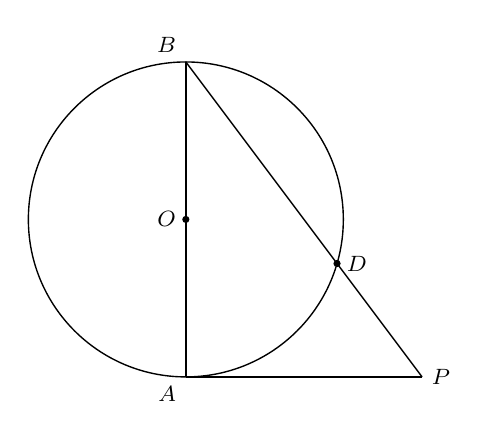
\begin{tikzpicture}[font=\footnotesize, line width=0.5pt, scale=1]
  \coordinate (O) at (0,0);
  \coordinate (A) at (0,-2);
  \coordinate (B) at (0,2);
  \coordinate (P) at (3,-2);
  \coordinate (D) at (1.92,-0.56);
  % 圆
  \draw (O) circle (2);
  % 直径 AB
  \draw (A) -- (B);
  % 切线 PA 与割线 PB
  \draw (P) -- (A);
  \draw (P) -- (B);
  % 点
  \fill (O) circle (1.3pt);
  \fill (D) circle (1.3pt);
  \node[left] at (O) {$O$};
  \node[below left] at (A) {$A$};
  \node[above left] at (B) {$B$};
  \node[right] at (P) {$P$};
  \node[right] at (D) {$D$};
\end{tikzpicture}
\end{center}
\nopagebreak[4]
\end{question}
\begin{question}
\gkti{12}将序号分别为 $1$，$2$，$3$，$4$，$5$ 的 $5$ 张参观券全部分给 $4$ 人，每人至少 $1$ 张，如果分给同一人的 $2$ 张参观券连号，那么不同的分法种数是\gkblank{}。

\Needspace{0.4\textheight}
\end{question}
\begin{question}
\gkti{13}向量 $\boldsymbol a$，$\boldsymbol b$，$\boldsymbol c$ 在正方形网格中的位置如图所示，若 $\boldsymbol c=\lambda\boldsymbol a+\mu\boldsymbol b$（$\lambda$，$\mu\in\mathbf R$），则 $\dfrac{\lambda}{\mu}=$\gkblank{}。
\nopagebreak[4]
\begin{center}% 2013 年北京卷理科第 13 题：正方形网格中的向量 a，b，c。
% 来源 PDF：普通高考/2013/2013北京理.pdf，第 1 页（印面 787）中栏。
% 网格 8×4；a 由 (2,0) 指向 (1,1)，b 由 (1,1) 指向 (7,3)，
% c 由 (7,3) 指向 (6,0)，故 a=(-1,1)，b=(6,2)，c=(-1,-3)。
\begin{tikzpicture}[font=\footnotesize, line width=0.4pt, scale=0.62]
  % 正方形网格
  \draw[step=1, gray!70] (0,0) grid (8,4);
  \draw[line width=0.6pt] (0,0) rectangle (8,4);
  % 向量 b
  \draw[->, line width=1.1pt, >=Stealth] (1,1) -- (7,3);
  % 向量 a
  \draw[->, line width=1.1pt, >=Stealth] (2,0) -- (1,1);
  % 向量 c
  \draw[->, line width=1.1pt, >=Stealth] (7,3) -- (6,0);
  % 标签
  \node at (0.92,0.62) {$a$};
  \node[above] at (4.1,2.35) {$b$};
  \node[right] at (6.62,1.45) {$c$};
\end{tikzpicture}
\end{center}
\nopagebreak[4]
\Needspace{0.4\textheight}
\end{question}
\begin{question}
\gkti{14}如图，在棱长为 $2$ 的正方体 $ABCD-A_1B_1C_1D_1$ 中，$E$ 为 $BC$ 的中点，点 $P$ 在线段 $D_1E$ 上，点 $P$ 到直线 $CC_1$ 的距离的最小值为\gkblank{}。
\nopagebreak[4]
\begin{center}% 2013 年北京卷理科第 14 题：棱长为 2 的正方体 ABCD-A1B1C1D1。
% 来源 PDF：普通高考/2013/2013北京理.pdf，第 1 页（印面 787）中栏。
% E 为 BC 的中点，P 在线段 D1E 上。
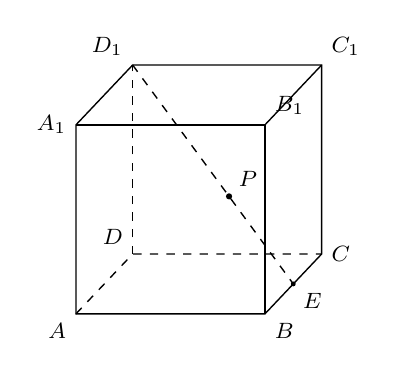
\begin{tikzpicture}[font=\footnotesize, line width=0.5pt, scale=0.8]
  % 前面 ABB1A1
  \coordinate (A) at (0,0);
  \coordinate (B) at (3,0);
  \coordinate (A1) at (0,3);
  \coordinate (B1) at (3,3);
  % 后面 DCC1D1（斜二测方向）
  \coordinate (D) at (0.9,0.95);
  \coordinate (C) at (3.9,0.95);
  \coordinate (C1) at (3.9,3.95);
  \coordinate (D1) at (0.9,3.95);
  % E 为 BC 中点
  \coordinate (E) at (3.45,0.475);
  % P 在线段 D1E 上
  \coordinate (P) at (2.43,1.865);
  % 可见棱
  \draw (A) -- (B) -- (C) -- (C1) -- (D1) -- (A1) -- cycle;
  \draw (A1) -- (B1) -- (B);
  \draw (B1) -- (C1);
  \draw (C) -- (C1);
  % 被遮挡的棱
  \draw[dashed] (A) -- (D) -- (C);
  \draw[dashed] (D) -- (D1);
  % 线段 D1E 与点 P
  \draw[dashed] (D1) -- (E);
  \fill (P) circle (1.4pt);
  \fill (E) circle (1.1pt);
  % 标签
  \node[below left] at (A) {$A$};
  \node[below right] at (B) {$B$};
  \node[right] at (C) {$C$};
  \node[above left] at (D) {$D$};
  \node[left] at (A1) {$A_1$};
  \node[above right] at (B1) {$B_1$};
  \node[above right] at (C1) {$C_1$};
  \node[above left] at (D1) {$D_1$};
  \node[below right] at (E) {$E$};
  \node[above right] at (P) {$P$};
\end{tikzpicture}
\end{center}
\nopagebreak[4]
\end{question}
\begingroup
\renewcommand{\gkpart}[1]{\Needspace{0.3\textheight}\subsection*{#1}\nopagebreak}
\gkpart{三、解答题}
\endgroup

\begin{question}
\gkti{15}在 $\triangle ABC$ 中，$a=3$，$b=2\sqrt6$，$\angle B=2\angle A$。

（1） 求 $\cos A$ 的值；

（2） 求 $c$ 的值。

\Needspace{0.4\textheight}
\end{question}
\begin{question}
\gkti{16}下图是某市 $3$ 月 $1$ 日至 $14$ 日的空气质量指数趋势图，空气质量指数小于 $100$ 表示空气质量优良，空气质量指数大于 $200$ 表示空气重度污染。某人随机选择 $3$ 月 $1$ 日至 $3$ 月 $13$ 日中的某一天到达该市，并停留 $2$ 天。
\nopagebreak[4]
\begin{center}% 2013 年北京卷理科第 16 题：3 月 1 日至 14 日空气质量指数趋势图。
% 来源 PDF：普通高考/2013/2013北京理.pdf，第 1 页（印面 787）右栏。
% 14 个数据点（600 dpi 原页逐个核对）：86，25，57，143，220，160，40，
% 217，160，121，158，86，79，37。
\begin{tikzpicture}[font=\scriptsize, >=Stealth, line width=0.45pt,
  x=0.79cm, y=0.026cm]
  % 坐标轴
  \draw[->] (0,0) -- (14.7,0);
  \node[below right] at (14.7,0) {日期};
  \draw[->] (0,0) -- (0,285) node[above] {空气质量指数};
  % 纵轴刻度与虚线
  \foreach \y in {50,100,150,200,250} {
    \draw (0,\y) -- (-0.12,\y) node[left] {\y};
    \draw[dashed, gray!55] (0,\y) -- (14.55,\y);
  }
  \node[below left] at (0,0) {$0$};
  % 横轴日期
  \foreach \i in {1,...,14} \node[below, font=\tiny] at (\i,0) {\i 日};
  % 数据折线与数据点
  \foreach \i/\v in {1/86,2/25,3/57,4/143,5/220,6/160,7/40,
                     8/217,9/160,10/121,11/158,12/86,13/79,14/37}
    \fill (\i,\v) circle (1.2pt);
  \draw (1,86) -- (2,25) -- (3,57) -- (4,143) -- (5,220) -- (6,160)
        -- (7,40) -- (8,217) -- (9,160) -- (10,121) -- (11,158)
        -- (12,86) -- (13,79) -- (14,37);
  % 数值标注
  \node[above left] at (1,86) {86};
  \node[left] at (2,25) {25};
  \node[above left] at (3,57) {57};
  \node[above] at (4,143) {143};
  \node[left] at (5,220) {220};
  \node[above left] at (6,160) {160};
  \node[above left] at (7,40) {40};
  \node[right] at (8,217) {217};
  \node[above left] at (9,160) {160};
  \node[left] at (10,121) {121};
  \node[above] at (11,158) {158};
  \node[below left] at (12,86) {86};
  \node[right] at (13,79) {79};
  \node[above left] at (14,37) {37};
\end{tikzpicture}
\end{center}
\nopagebreak[4]
（1） 求此人到达当日空气重度污染的概率；

（2） 设 $X$ 是此人停留期间空气质量优良的天数，求 $X$ 的分布列与数学期望；

（3） 由图判断从哪天开始连续三天的空气质量指数方差最大？（结论不要求证明）

\Needspace{0.4\textheight}
\end{question}
\begin{question}
\gkti{17}如图，在三棱柱 $ABC-A_1B_1C_1$ 中，$AA_1C_1C$ 是边长为 $4$ 的正方形。平面 $ABC\perp$ 平面 $AA_1C_1C$，$AB=3$，$BC=5$。

（1） 求证：$AA_1\perp$ 平面 $ABC$；

（2） 求二面角 $A_1-BC_1-B_1$ 的余弦值；

（3） 证明：在线段 $BC_1$ 上存在点 $D$，使得 $AD\perp A_1B$，并求 $\dfrac{BD}{BC_1}$ 的值。
\nopagebreak[4]
\begin{center}% 2013 年北京卷理科第 17 题：三棱柱 ABC-A1B1C1。
% 来源 PDF：普通高考/2013/2013北京理.pdf，第 2 页（印面 788）左栏。
% AA1C1C 是边长为 4 的正方形，平面 ABC⊥平面 AA1C1C，AB=3，BC=5。
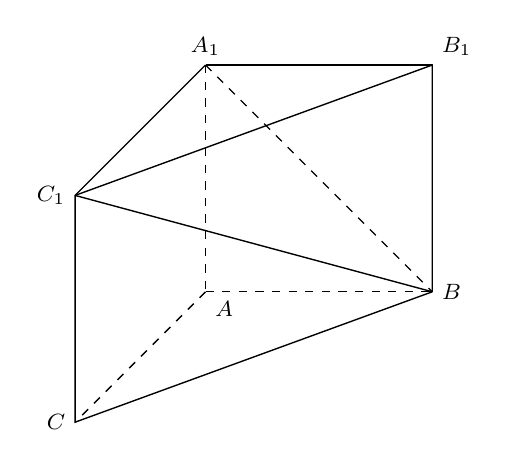
\begin{tikzpicture}[font=\footnotesize, line width=0.5pt, scale=0.72]
  % 正方形侧面 AA1C1C（平行四边形画法）：A1 在上，C1 在左上，A 在下，C 在左下
  \coordinate (A1) at (0,0);
  \coordinate (C1) at (-2.3,-2.3);
  \coordinate (A)  at (0,-4.0);
  \coordinate (C)  at (-2.3,-6.3);
  % AB 垂直于侧面，B 在右前方
  \coordinate (B)  at (4.0,-4.0);
  \coordinate (B1) at (4.0,0);
  % 可见棱
  \draw (A1) -- (C1) -- (C) -- (B);
  \draw (C1) -- (B1) -- (B);
  \draw (A1) -- (B1);
  % 被遮挡的棱
  \draw[dashed] (A1) -- (A);
  \draw[dashed] (A) -- (C);
  \draw[dashed] (A) -- (B);
  % 辅助线 A1B、C1B
  \draw[dashed] (A1) -- (B);
  \draw (C1) -- (B);
  % 顶点标签
  \node[above] at (A1) {$A_1$};
  \node[left] at (C1) {$C_1$};
  \node[above right] at (B1) {$B_1$};
  \node[below right] at (A) {$A$};
  \node[right] at (B) {$B$};
  \node[left] at (C) {$C$};
\end{tikzpicture}
\end{center}
\nopagebreak[4]
\end{question}
\begin{question}
\gkti{18}设 $L$ 为曲线 $C:y=\dfrac{\ln x}{x}$ 在点 $(1,0)$ 处的切线。

（1） 求 $L$ 的方程；

（2） 证明：除切点 $(1,0)$ 之外，曲线 $C$ 在直线 $L$ 的下方。

\end{question}
\begin{question}
\gkti{19}已知 $A$，$B$，$C$ 是椭圆 $W:\dfrac{x^2}4+y^2=1$ 上的三个点，$O$ 是坐标原点。

（1） 当点 $B$ 是 $W$ 的右顶点，且四边形 $OABC$ 为菱形时，求此菱形的面积；

（2） 当点 $B$ 不是 $W$ 的顶点时，判断四边形 $OABC$ 是否可能为菱形，并说明理由。

\end{question}
\begin{question}
\gkti{20}已知 $\{a_n\}$ 是由非负整数组成的无穷数列，该数列前 $n$ 项的最大值记为 $A_n$，第 $n$ 项之后各项 $a_{n+1}$，$a_{n+2}$，$\cdots$ 的最小值记为 $B_n$，$d_n=A_n-B_n$。

（1） 若 $\{a_n\}$ 为 $2$，$1$，$4$，$3$，$2$，$1$，$4$，$3$，$\cdots$，是一个周期为 $4$ 的数列（即对任意 $n\in\mathbf N^*$，$a_{n+4}=a_n$），写出 $d_1$，$d_2$，$d_3$，$d_4$ 的值；

（2） 设 $d$ 是非负整数，证明：$d_n=-d$（$n=1$，$2$，$3$，$\cdots$）的充分必要条件为 $\{a_n\}$ 是公差为 $d$ 的等差数列；

（3） 证明：若 $a_1=2$，$d_n=1$（$n=1$，$2$，$3$，$\cdots$），则 $\{a_n\}$ 的项只能是 $1$ 或者 $2$，且有无穷多项为 $1$。

\end{question}